\documentclass[11pt]{article}
\usepackage{enumitem}
\usepackage{float}
\usepackage[margin=1in]{geometry}
\usepackage{graphicx}
\usepackage[space]{grffile}
\usepackage{adjustbox}
\usepackage{amsmath}
\usepackage{amsthm}
\usepackage{amssymb}
\usepackage{fullpage}
\usepackage{fancyhdr}
\usepackage{xparse}
\newcommand*{\boxtex}[1]{\framebox{#1}}
\newcommand{\cnum}{CM146}
\newcommand{\ced}{Fall 2018}
\newcommand{\ctitle}[3]{\title{\vspace{-0.5in}\cnum, \ced\\Problem Set #1: #2}}
\newcommand{\solution}[1]{{{\color{blue}{\bf Solution:} {#1}}}}
\NewDocumentCommand{\texcod}{mm}{%
	\texttt{\textcolor{#1}{#2}}%
}
\usepackage[usenames,dvipsnames,svgnames,table,hyperref]{xcolor}

\renewcommand*{\theenumi}{\alph{enumi}}
\renewcommand*\labelenumi{(\theenumi)}
\renewcommand*{\theenumii}{\roman{enumii}}
\renewcommand*\labelenumii{\theenumii.}

\author{Zheng Wang}
\date{\today}
\title{MATH 151A Homework 1}

\begin{document}
\maketitle

\section*{Question 1}
\begin{itemize}
	\item [(a)]
	First, I will show that the limit $ p^* $ is $ 0 $.\\
	Let $ g(x) = x - \frac{1}{2}\ln(x+1) $, Then we have $ g(0) = 0 $ and $ g'(x)= 1-\frac{1}{2}\cdot \frac{1}{x+1} \ge 0 \quad \forall x > 0 $. Since $ g $ and $ g' $ both exist and are continous, it follows from Mean Value Theorem that there exist $ \xi \in (0,x) $ such that $ g'(\xi) = \frac{g(x)-g(0)}{x-0} = \frac{g(x)}{x}$.
	So, $g(x) = x\cdot g'(\xi) \ge 0 $ and $ x \ge \frac{1}{2}\ln (x+1) $.\\
	\textbf{Claim:} $ 0 < p_n \le 2^{-n} $.\\
	\textit{proof.} First, $ 0 < p_1 \le 1 $. Then, suppose $ 0 < p_n \le 2^{-n} $, then, we have $ 0 < p_{n+1} = \frac{1}{2}\ln(p_n+1) \le \frac{1}{2}p_n \le 2^{-(n+1)} $. So, by induction, $ 0 < p_n \le 2^{-n} $ and it follows from squeeze theorem that $ \lim_{n \rightarrow \infty} p_n = p^* = 0 $.\\\\
	Then, compute the convergence order and asymptotic rate of convergence. 
	\[ \lim_{n\rightarrow \infty} \left| \frac{p_{n+1}}{(p_n)^\alpha} \right| = \lim_{p_n \rightarrow 0} \frac{\frac{1}{2}\ln(p_n + 1)}{p_n} \cdot \frac{1}{(p_n)^{\alpha -1}} = \frac{1}{2} \cdot \lim_{p_n \rightarrow 0} \frac{1}{(p_n)^{\alpha -1}} = \frac{1}{2} \quad\text{when } \alpha = 1 \]
	Thus, \boxtex{$ \alpha = 1 $} and \boxtex{$ \lambda = \frac{1}{2} $}, and the sequence converges linearly. \hfill $ \blacksquare $
	
	\item[(b)]
	First, I will show that the limit $ p^* $ is $ 1 $.\\
	We have \[ \lim_{n \rightarrow \infty} 1+ 2^{1-n} +\frac{1}{(n+2)^n} = 1+ \lim_{n \rightarrow \infty}2^{1-n} + \lim_{n \rightarrow \infty} \frac{1}{(n+2)^n} = 1+0+0 = 1 \]
	Thus, $ p^*  = 1$.\\\\
	Then, we show that the convergence is linear by compute $ \lambda $ and $ \alpha $ as follows:\\
	\begin{equation*}
	\begin{aligned}
	\lim_{n \rightarrow \infty} \left|\frac{p_{n+1} - 1}{(p_n-1)^\alpha}\right| &= \lim_{n \rightarrow \infty} \left|\frac{2^{-n}+\frac{1}{(n+3)^{n+1}}}{(2^{1-n} + \frac{1}{(n+2)^n})^\alpha}\right|\\
	&= \lim_{n \rightarrow \infty} \frac{2^{(\alpha-1)n} + \frac{2^{\alpha n}}{(n+3)^{n+1}}}{ \left(2 + \frac{2^n}{(n+2)^n} \right)^\alpha} \\
	&= \frac{\lim_{n \rightarrow \infty} 2^{(\alpha-1)n} + \lim_{n \rightarrow \infty} \frac{2^{\alpha n}}{(n+3)^{n+1}}}{ \left( 2 + \lim_{n \rightarrow \infty} \frac{2^n}{(n+2)^n} \right)^\alpha }\\
	&= \frac{\lim_{n \rightarrow \infty} 2 ^{(\alpha -1)n}}{2^\alpha} = \frac{1}{2} \quad \text{when } \alpha = 1
	\end{aligned}
	\end{equation*}
	Thus, \boxtex{$ \alpha = 1 $} and \boxtex{$ \lambda = \frac{1}{2} $}, and convergence is linear. \hfill $ \blacksquare $
\end{itemize}

\section*{Question 2}
First, we show that $ p^*  = 0$ since
\[ \lim_{n \rightarrow \infty} 10^{(-2^n)} = \lim_{n \rightarrow \infty} \left(10^{-1}\right)^{2^n} = \lim_{n \rightarrow \infty} \left( \frac{1}{10}\right)^{2^n}  = 0\]
Then, we have 
\[ \lim_{n \rightarrow \infty} \left|\frac{ \left(\frac{1}{10}\right)^{2^{n+1}} }{ \left( \left(\frac{1}{10}\right)^{2^{n}} \right)^\alpha }\right| = \lim_{n \rightarrow \infty} \left|\frac{ \left(\frac{1}{10}\right)^{2^{n}\cdot 2} }{  \left(\frac{1}{10}\right)^{2^{n}\cdot \alpha}  }\right| = \lim_{n \rightarrow \infty} \left| \left( \frac{1}{10}\right)^{(2-\alpha)\cdot 2^n} \right| = 1 \quad\text{when } \alpha = 2\] 
Thus, \boxtex{$ \alpha =2 $} and \boxtex{$ \lambda = 1 $}, so the sequence converges quadratically\hfill $ \blacksquare $

\section*{Question 3}
\begin{itemize}
	\item [(a)]
	By Lagrange interpolation, we have 
	\begin{equation*}
	\begin{aligned}
	P(x) &= f(1)\cdot\frac{(x-2)(x-3)(x-4)}{(1-2)(1-3)(1-4)} + f(2)\cdot\frac{(x-1)(x-3)(x-4)}{(2-1)(2-3)(2-4)} \\
	&+ f(3)\cdot\frac{(x-1)(x-2)(x-4)}{(3-1)(3-2)(3-4)} + f(4)\cdot\frac{(x-1)(x-2)(x-3)}{(4-1)(4-2)(4-3)}\\
	&=-\frac{4}{3}x^3+10x^2-\frac{65}{3}x+15
	\end{aligned}
	\end{equation*}
	Thus, we have \boxtex{$ f(x)= -\frac{4}{3}x^3+10x^2-\frac{65}{3}x+15 $}
	
	\item[(b)]
	At the first iteration of Neville's Method, we have the following:
	\[ P_0 = f(x_0) = f(1)=2 \quad\quad P_1 = f(x_1) = f(2)=1 \]
	\[ P_2 = f(x_2) = f(3)=4 \quad\quad P_3 = f(x_3) = f(4)=3 \]
	At the second iteration of Neville's Method, we have the following:
	\[ P_{0,1} = \frac{(x-2)P_0 - (x-1)P_1}{1-2} = 3-x\]
	\[ P_{1,2} = \frac{(x-3)P_1 - (x-2)P_2}{2-3} = 3x-5\]
	\[ P_{2,3} = \frac{(x-4)P_2 - (x-3)P_3}{3-4} = 7-x\]
	At the third iteration of Neville's Method, we have the following:
	\[ P_{0,1,2} = \frac{(x-3)P_{0,1} - (x-1)P_{1,2} }{1-3} = 2x^2-7x+7\]
	\[ P_{1,2,3} = \frac{(x-4)P_{1,2} - (x-2)P_{2,3} }{2-4} = -2x^2+13x-17\]
	Finally, Nevilles' Method give us the ultimate polynomial:
	\[ P_{0,1,2,3} = \frac{ (x-4)P_{0,1,2} - (x-1)P_{1,2,3}  }{1-4}  = -\frac{4}{3}x^3+10x^2-\frac{65}{3}x+15 \]
	Thus, we have \boxtex{$ f(x)= -\frac{4}{3}x^3+10x^2-\frac{65}{3}x+15 $} from Neville's Method.
\end{itemize}

\section*{Question 4 (Coding)}
\begin{itemize}
	\item [(a)]
	I obtain the following graph from MATLAB:\\
	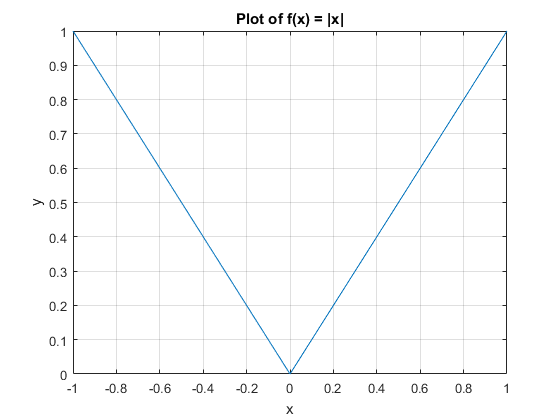
\includegraphics{abs_x_plot.png}
	
	\item [(b)]
	I obtain the following graph from MATLAB:\\
	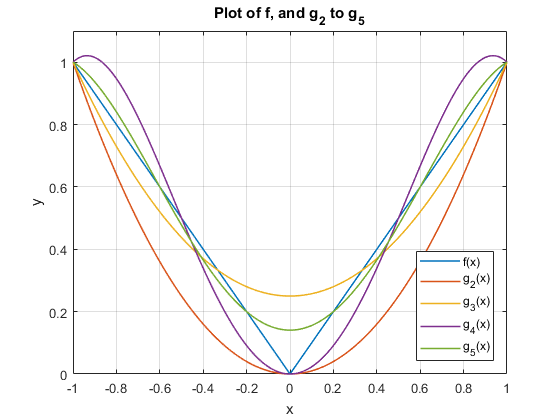
\includegraphics{g_2_to_g_5.png}\pagebreak
	
	\item[(c)]
	I obtain the following graph:\\
	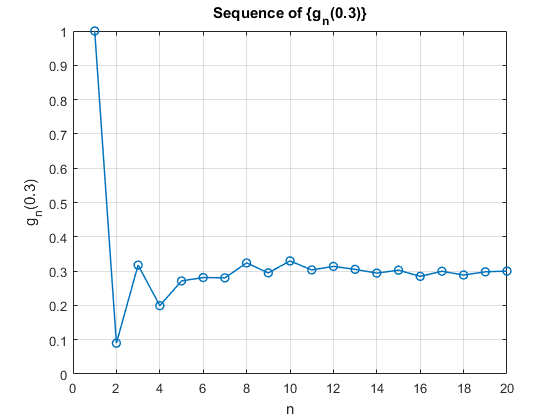
\includegraphics{g_n_seq.png}\pagebreak
\end{itemize}

\section*{Code for question 4}
\begin{verbatim}
% % MATH 151A HOMEWORK 2
% % QUESTION 4
% % Wang, Zheng
% % Results are recorded in homework2.pdf

%% (a) plot the graph
figure;
fplot(@f, [-1,1]);
xlabel('x');
ylabel('y');
title('Plot of f(x) = |x|');
grid on;

%% (b) Plot 
sequence(5)
figure;
fplot(@f, [-1,1],'Linewidth', 1.1);
hold on;

for g=2:5
    [fx,x] = plt_seq(solv(sequence(g),f(sequence(g))));
    plot(fx,x,'Linewidth', 1.1)
end

xlabel('x');
ylabel('y');
legend({'f(x)','g_2(x)', 'g_3(x)','g_4(x)','g_5(x)'},'Location','southeast')
title('Plot of f, and g_2 to g_5');
grid on;
hold off;

%% (c) sequence of g_n
result = ones(1,20);
for n=1:20
    result(1,n) = eval_func( solv(sequence(n),f(sequence(n))) );
end

figure;
plot(1:20, result, 'o-', 'Linewidth', 1.1);
xlabel('n');
ylabel('g_n(0.3)');
title('Sequence of \{g_n(0.3)\}');
grid on;

%% Function declaration
function y = f(x)
    y = abs(x);
end

function x_nk = sequence(n)
    x_nk_t = ones(n+1,1);
    for k=0:n
        x_nk_t(k+1,1) = -1 + (2*k)/n;
    end
    x_nk = x_nk_t;
end

function coef = solv(x, y)
    n = size(x,1);
    X = repmat(x,1,n);
    for j=1:n
        X(:,j) = X(:,j).^(j-1);
    end
    coef = X\y;
end

function [x, fx] = plt_seq(coef)
    x = sequence(100);
    degree = size(coef,1);
    X = repmat(x,1,degree);
    for i=1:degree
        X(:,i) = X(:,i).^(i-1);
    end
    fx = X*coef;
    x = x';
    fx = fx';
end

function fx = eval_func(coef)
    x = 0.3;
    degree = size(coef,1);
    X = repmat(x,1,degree);
    for i=1:degree
        X(:,i) = X(:,i).^(i-1);
    end
    fx = X*coef;
end 
\end{verbatim}
\end{document}